% Options for packages loaded elsewhere
\PassOptionsToPackage{unicode,linktoc=all}{hyperref}
\PassOptionsToPackage{hyphens}{url}
\PassOptionsToPackage{dvipsnames,svgnames,x11names}{xcolor}
%
\documentclass[
  a4paper,
]{article}
\usepackage{amsmath,amssymb}
\usepackage{iftex}
\ifPDFTeX
  \usepackage[T1]{fontenc}
  \usepackage[utf8]{inputenc}
  \usepackage{textcomp} % provide euro and other symbols
\else % if luatex or xetex
  \usepackage{unicode-math} % this also loads fontspec
  \defaultfontfeatures{Scale=MatchLowercase}
  \defaultfontfeatures[\rmfamily]{Ligatures=TeX,Scale=1}
\fi
\usepackage{lmodern}
\ifPDFTeX\else
  % xetex/luatex font selection
\fi
% Use upquote if available, for straight quotes in verbatim environments
\IfFileExists{upquote.sty}{\usepackage{upquote}}{}
\IfFileExists{microtype.sty}{% use microtype if available
  \usepackage[]{microtype}
  \UseMicrotypeSet[protrusion]{basicmath} % disable protrusion for tt fonts
}{}
\makeatletter
\@ifundefined{KOMAClassName}{% if non-KOMA class
  \IfFileExists{parskip.sty}{%
    \usepackage{parskip}
  }{% else
    \setlength{\parindent}{0pt}
    \setlength{\parskip}{6pt plus 2pt minus 1pt}}
}{% if KOMA class
  \KOMAoptions{parskip=half}}
\makeatother
\usepackage{xcolor}
\usepackage[margin=25mm]{geometry}
\usepackage{longtable,booktabs,array}
\usepackage{calc} % for calculating minipage widths
% Correct order of tables after \paragraph or \subparagraph
\usepackage{etoolbox}
\makeatletter
\patchcmd\longtable{\par}{\if@noskipsec\mbox{}\fi\par}{}{}
\makeatother
% Allow footnotes in longtable head/foot
\IfFileExists{footnotehyper.sty}{\usepackage{footnotehyper}}{\usepackage{footnote}}
\makesavenoteenv{longtable}
\usepackage{graphicx}
\makeatletter
\def\maxwidth{\ifdim\Gin@nat@width>\linewidth\linewidth\else\Gin@nat@width\fi}
\def\maxheight{\ifdim\Gin@nat@height>\textheight\textheight\else\Gin@nat@height\fi}
\makeatother
% Scale images if necessary, so that they will not overflow the page
% margins by default, and it is still possible to overwrite the defaults
% using explicit options in \includegraphics[width, height, ...]{}
\setkeys{Gin}{width=\maxwidth,height=\maxheight,keepaspectratio}
% Set default figure placement to htbp
\makeatletter
\def\fps@figure{htbp}
\makeatother
\usepackage{svg}
\setlength{\emergencystretch}{3em} % prevent overfull lines
\providecommand{\tightlist}{%
  \setlength{\itemsep}{0pt}\setlength{\parskip}{0pt}}
\setcounter{secnumdepth}{-\maxdimen} % remove section numbering
% definitions for citeproc citations
\NewDocumentCommand\citeproctext{}{}
\NewDocumentCommand\citeproc{mm}{%
  \begingroup\def\citeproctext{#2}\cite{#1}\endgroup}
\makeatletter
 % allow citations to break across lines
 \let\@cite@ofmt\@firstofone
 % avoid brackets around text for \cite:
 \def\@biblabel#1{}
 \def\@cite#1#2{{#1\if@tempswa , #2\fi}}
\makeatother
\newlength{\cslhangindent}
\setlength{\cslhangindent}{1.5em}
\newlength{\csllabelwidth}
\setlength{\csllabelwidth}{3em}
\newenvironment{CSLReferences}[2] % #1 hanging-indent, #2 entry-spacing
 {\begin{list}{}{%
  \setlength{\itemindent}{0pt}
  \setlength{\leftmargin}{0pt}
  \setlength{\parsep}{0pt}
  % turn on hanging indent if param 1 is 1
  \ifodd #1
   \setlength{\leftmargin}{\cslhangindent}
   \setlength{\itemindent}{-1\cslhangindent}
  \fi
  % set entry spacing
  \setlength{\itemsep}{#2\baselineskip}}}
 {\end{list}}
\usepackage{calc}
\newcommand{\CSLBlock}[1]{\hfill\break\parbox[t]{\linewidth}{\strut\ignorespaces#1\strut}}
\newcommand{\CSLLeftMargin}[1]{\parbox[t]{\csllabelwidth}{\strut#1\strut}}
\newcommand{\CSLRightInline}[1]{\parbox[t]{\linewidth - \csllabelwidth}{\strut#1\strut}}
\newcommand{\CSLIndent}[1]{\hspace{\cslhangindent}#1}
\ifLuaTeX
\usepackage[bidi=basic]{babel}
\else
\usepackage[bidi=default]{babel}
\fi
\babelprovide[main,import]{british}
% get rid of language-specific shorthands (see #6817):
\let\LanguageShortHands\languageshorthands
\def\languageshorthands#1{}
% $HOME/.pandoc/defaults/latex-header-includes.tex
% Common header includes for both lualatex and xelatex engines.
%
% Preliminaries
%
% \PassOptionsToPackage{rgb,dvipsnames,svgnames}{xcolor}
% \PassOptionsToPackage{main=british}{babel}
\PassOptionsToPackage{english}{selnolig}
\AtBeginEnvironment{quote}{\small}
\AtBeginEnvironment{quotation}{\small}
\AtBeginEnvironment{longtable}{\centering}
%
% Packages that are useful to include
%
\usepackage{graphicx}
\usepackage{subcaption}
\usepackage[inkscapeversion=1]{svg}
\usepackage[defaultlines=4,all]{nowidow}
\usepackage{etoolbox}
\usepackage{fontsize}
\usepackage{newunicodechar}
\usepackage{pdflscape}
\usepackage{fnpct}
\usepackage{parskip}
  \setlength{\parindent}{0pt}
\usepackage[style=american]{csquotes}
% \usepackage{setspace} Use the <fontname-plus.tex> files for setspace
%
\usepackage{hyperref} % cleveref must come AFTER hyperref
\usepackage[capitalize,noabbrev]{cleveref} % Must come after hyperref
\let\longdivision\relax
\usepackage{longdivision}
% noto-plus.tex
% Font-setting header file for use with Pandoc Markdown
% to generate PDF via LuaLaTeX.
% The main font is Noto Serif.
% Other main fonts are also available in appropriately named file.
\usepackage{fontspec}
\usepackage{setspace}
\setstretch{1.3}
%
\defaultfontfeatures{Ligatures=TeX,Scale=MatchLowercase,Renderer=Node} % at the start always
%
% For English
% See also https://tex.stackexchange.com/questions/574047/lualatex-amsthm-polyglossia-charissil-error
% We use Node as Renderer for the Latin Font and Greek Font and HarfBuzz as renderer ofr Indic fonts.
%
\babelfont{rm}[Script=Latin,Scale=1]{NotoSerif}% Config is at $HOME/texmf/tex/latex/NotoSerif.fontspec
\babelfont{sf}[Script=Latin]{SourceSansPro}% Config is at $HOME/texmf/tex/latex/SourceSansPro.fontspec
\babelfont{tt}[Script=Latin]{FiraMono}% Config is at $HOME/texmf/tex/latex/FiraMono.fontspec
%
% Sanskrit, Tamil, and Greek fonts
%
\babelprovide[import, onchar=ids fonts]{sanskrit}
\babelprovide[import, onchar=ids fonts]{tamil}
\babelprovide[import, onchar=ids fonts]{greek}
%
\babelfont[sanskrit]{rm}[Scale=1.1,Renderer=HarfBuzz,Script=Devanagari]{NotoSerifDevanagari}
\babelfont[sanskrit]{sf}[Scale=1.1,Renderer=HarfBuzz,Script=Devanagari]{NotoSansDevanagari}
\babelfont[tamil]{rm}[Renderer=HarfBuzz,Script=Tamil]{NotoSerifTamil}
\babelfont[tamil]{sf}[Renderer=HarfBuzz,Script=Tamil]{NotoSansTamil}
\babelfont[greek]{rm}[Script=Greek]{GentiumBookPlus}
%
% Math font
%
\usepackage{unicode-math} % seems not to hurt % fallabck
\setmathfont[bold-style=TeX]{STIX Two Math}
\usepackage{amsmath}
\usepackage{esdiff} % for derivative symbols
% \renewcommand{\mathbf}{\symbf}
%
%
% Other fonts
%
\newfontfamily{\emojifont}{Symbola}
%

\usepackage{titling}
\usepackage{fancyhdr}
    \pagestyle{fancy}
    \fancyhead{}
    \fancyfoot{}
    \renewcommand{\headrulewidth}{0.2pt}
    \renewcommand{\footrulewidth}{0.2pt}
    \fancyhead[LO,RE]{\scshape\thetitle}
    \fancyfoot[CO,CE]{\footnotesize Copyright © 2006\textendash\the\year, R (Chandra) Chandrasekhar}
    \fancyfoot[RE,RO]{\thepage}
%
\usepackage{newunicodechar}
\newunicodechar{√}{\textsf{√}}
\ifLuaTeX
  \usepackage{selnolig}  % disable illegal ligatures
\fi
\usepackage{bookmark}
\IfFileExists{xurl.sty}{\usepackage{xurl}}{} % add URL line breaks if available
\urlstyle{sf}
\hypersetup{
  pdftitle={Doron's Mathematical Amnesia},
  pdfauthor={R (Chandra) Chandrasekhar},
  pdflang={en-GB},
  colorlinks=true,
  linkcolor={DarkOliveGreen},
  filecolor={Purple},
  citecolor={DarkKhaki},
  urlcolor={Maroon},
  pdfcreator={LaTeX via pandoc}}

\title{Doron's Mathematical Amnesia}
\author{R (Chandra) Chandrasekhar}
\date{2024-04-08 | 2024-04-10}

\begin{document}
\maketitle

\thispagestyle{empty}


``I don't know if you have heard, but my dear friend Doron Rabinovich
met with a rather bad accident about two weeks ago. Thankfully, it was
not fatal, but he did suffer a very severe concussion,'' my friend Solus
``Sol'' Simkin told me, as we settled for a leisurely afternoon tea at
our favourite \href{http://www.orchardvalleycoffee.net/}{\emph{Orchard
Valley Coffeeshop}}.

``I don't know Doron well, but I do recall that he had quite a way with
numbers,'' I replied.

``Poor Doron has suffered a strange cognitive deficit. His language and
speech skills have survived intact, but he has developed `selective
mathematical amnesia'. He has forgotten much of high school
mathematics---which for a person with a Master's degree in
engineering---is a rather tragic state of affairs. In fact, his
knowledge of mathematics now resembles
\href{https://en.wikipedia.org/wiki/Emmental_cheese}{Emmental
cheese}---full of holes.''

\begin{figure}
\centering
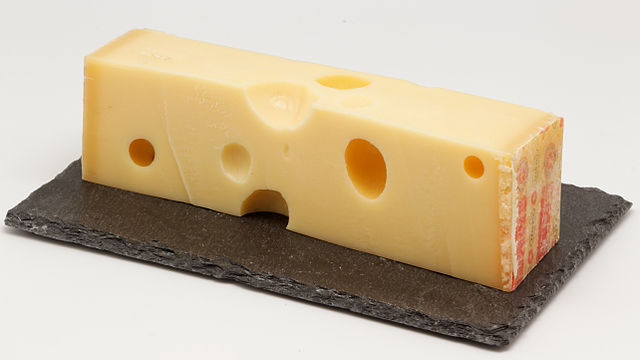
\includegraphics[width=0.7\textwidth,height=\textheight]{images/emmental-cheese.jpg}
\caption[Emmental cheese is full of holes.]{Emmental cheese is full of
holes.\footnotemark{}}\label{fig:cheese}
\end{figure}
\footnotetext{Attribution: Coyau /
  \href{https://commons.wikimedia.org/wiki/Main_Page}{Wikimedia Commons}
  / \href{https://creativecommons.org/licenses/by-sa/3.0/}{CC BY-SA 3.0}}

``Indeed,'' I replied. ``Is there any way out?''

``Come to think of it, most youngsters' knowledge of mathematics also
resembles Emmental cheese nowadays. Their attention spans are so
short-lived, and their memories so volatile, that many of them belatedly
discover that they also suffer from mathematical amnesia when they enter
university.

``I thought it a good idea to see if I could help repair and restore
Doron's recollection of mathematics, and have embarked on an effort to
that end. Who knows, many school leavers could also find the programme
useful.''

``Tell me more,'' I quipped, and settled down to yet another Simkin Tale
as Sol recounted his adventure with Doron. The rest of this blog is the
verbatim first person account of Sol.

\subsection{To heal amnesia, start with
history}\label{to-heal-amnesia-start-with-history}

``I strongly believe that to heal amnesia, we must start with history.
The networked tapestry of history is a durable foundation upon which to
recollect, repair, and restore. It will be an insurance against future
selective amnesia.

``Accordingly, I started Doron on the third edition of John Stillwell's
book,
\href{https://www.amazon.in/Mathematics-Its-History-Undergraduate-Texts/dp/144196052X}{Mathematics
and Its History} {[}\citeproc{ref-stillwell2010}{1}{]}.''

\begin{figure}
\centering

\includegraphics[width=0.5\textwidth,height=\textheight]{images/stillwell-history-third.jpg}
\caption{The third edition of John Stillwell's \emph{Mathematics and Its
History}.}\label{fig:stillwell}
\end{figure}

``I told him to read it through, with or without full comprehension. I
asked him to gloss over the problems. I promised that I would direct
Doron to tractable problems. He would then make some effort remembering,
and sketching a solution. I would guide him if he got stuck. It seemed
to me to be a workable compromise between spoonfeeding and letting him
drown at the deep end.''

\subsection{A trigonometric identity from
yesteryear}\label{a-trigonometric-identity-from-yesteryear}

Between pages 7 and 9 of his book, Stillwell gives clues aplenty, for
problem 1.3.4, to guide a student into discovering expressions for
\(\cos\theta\) and \(\sin\theta\) in terms of
\(t = \tan\frac{\theta}{2}\):
\begin{equation}\phantomsection\label{eq:costheta}{
\cos\theta = \frac{1 - t^2}{1 + t^2}
}\end{equation} and \begin{equation}\phantomsection\label{eq:sintheta}{
\sin\theta = \frac{2t}{1 + t^2}
}\end{equation}

I asked Doron to attempt this rather ancient problem, but he greeted me
with eyes glazed by incomprehension. I felt really sorry for the poor
sod, and determined that I would handhold him for at least this problem.

\subsection{Starting with the unit
circle}\label{starting-with-the-unit-circle}

This is a problem that is most easily understood using diagrams. I
thought that Doron's face would light up in an instant once he saw
\cref{fig:pythagoras}. Alas! I was mistaken. Here is the image that I
first showed him:

\begin{figure}
\centering
\includesvg[width=0.9\textwidth,height=\textheight]{images/pythagoras.svg}
\caption{A right triangle on a unit circle. See the text for the
discussion.}\label{fig:pythagoras}
\end{figure}

It elicited almost no indication of knowingness from Doron. He simply
stared blankly at it. That was when I realized that the diagrams of
mathematics, which hold such significance for the cognoscenti, are
simply meaningless scrawls of black on white for the vast untutored
majority. And I was aghast that my dear Doron had joined their numbers
now. But, I soldiered on.

``Let us assume the truth of the
\href{https://en.wikipedia.org/wiki/Pythagorean_theorem}{Pythagorean
theorem}'', I told Doron. ``In \cref{fig:pythagoras}, we have a circle
with centre \(O\) and a radius of one, also called a unit circle. The
triangle \(OPR\) is right-angled and \(R\) is an arbitrary point on the
circle, having coordinates \((x, y)\). Note that the radius \(OR\) is
one unit in length. By the theorem of Pythagoras, we may claim that
\begin{equation}\phantomsection\label{eq:circle}{
\begin{aligned}
OP^2 + PR^2 &= OR^2\\
x^2 + y^2 &= 1.
\end{aligned}
}\end{equation} This is also the equation of the circle.''

Interestingly, because the hypotenuse is one unit, we may also say that
\(\cos\theta = \frac{x}{1} = x\) and similarly that
\(\sin\theta = \frac{y}{1} = y\). Moreover, \(\tan\theta = \frac{y}{x}\)
by definition. All these formulae are also included in
\cref{fig:pythagoras} in order to stimulate recollection. In a polite
gesture devoid of intelligence, Doron nodded like a dazed man. It was
gut-wrenching to see such steep intellectual decline in one who was once
so brilliant.

\subsection{\texorpdfstring{Getting to
\(\tan\frac{\theta}{2}\)}{Getting to \textbackslash tan\textbackslash frac\{\textbackslash theta\}\{2\}}}\label{getting-to-tanfractheta2}

Suppressing my doubts as to whether it was worthwhile to proceed
further, I battled on. I showed Doron \cref{fig:tantheta}, and told him
that here we needed some geometry and the ability to solve
\href{https://en.wikipedia.org/wiki/Quadratic_equation}{quadratic
equations}. The moment he heard the word \emph{quadratic}, Doron perked
up a little, buoyed perhaps by a memory of an early mathematical triumph
from his schooldays.

\begin{figure}
\centering
\includesvg[width=0.9\textwidth,height=\textheight]{images/tantheta.svg}
\caption{\(\cos\theta\) and \(\sin\theta\) vis-a-vis
\(\tan\frac{\theta}{2}\). See the text for
explanation.}\label{fig:tantheta}
\end{figure}

We now draw a line from \(Q\) to \(R\), which intersects the \(y\) axis
at \(S(0, t)\). Looking at triangle \(OQR\), it is clear that that its
two legs, \(OQ\) and \(OR\), are equal since they are both radii of the
unit circle.

I now believed that I had Doron's attention, and decided to pounce for
the kill. I asked Doron if he could tell me something about
\href{https://en.wikipedia.org/wiki/Isosceles_triangle}{isosceles
triangles} in which the two legs were equal. Startlingly, he said ``same
base angles''. I was incredibly encouraged.

Let us call these equal angles \(\alpha\) as marked on
\cref{fig:tantheta}. ``How are the values \(\alpha\) and \(\theta\)
related?'' I ventured next. ``Think about the properties of triangles in
elementary school. What is a property common to \emph{all triangles},
not only isosceles ones?''

Doron stared vacantly again. I decided to let him rest his injured
brain, and resume his mathematical rehabilitation another day.

\subsection{The exterior angle of a
triangle}\label{the-exterior-angle-of-a-triangle}

When we resumed two days later, Doron struggled to say a word. He
started out ``ext, ext, ext'' but could not go further. It was then that
I realized how important are the \emph{names} we attach to concepts and
things. The very basis of all knowledge is to able to name new objects.
Only then can we progress to know about them. In his heroic struggle,
Doron had reached the doorstep of the correct name, but could not open
the door.

``How about exterior angle, Doron?'' I asked. I was rewarded with a
``Yes, yes, yes, yes.'' With a little more nudging, we got to the point
where Doron remembered that
\href{https://www.storyofmathematics.com/exterior-angle-theorem/}{the
exterior angle of a triangle equalled the sum of its two interior
angles}.

I slowly coaxed Doron along until he could utter ``Alpha is half
theta''. That I considered a major breakthrough, for indeed,
\begin{equation}\phantomsection\label{eq:alpha}{
\alpha = \frac{\theta}{2}.
}\end{equation} Doron proudly told me that he did not need the help of
the statement \(\theta = 2\alpha\) shown in \cref{fig:tantheta} to work
this out. I was beside myself with happiness and decided then to
punctuate my rehabilitation sessions with generous periods of rest,
until Doron started consistently remembering what he already once knew.

\subsection{\texorpdfstring{What does \(\tan\alpha\) equal
to?}{What does \textbackslash tan\textbackslash alpha equal to?}}\label{what-does-tanalpha-equal-to}

At the next session, I asked Doron to concentrate on triangle \(OQS\).
Stillwell had astutely suggested in his book that \(OS\) should be set
to some parameter \(t\). By definition then, because \(OQ\) is a radius,
\begin{equation}\phantomsection\label{eq:halftheta}{
\tan\alpha = \tan\frac{\theta}{2} = \frac{OS}{OQ} = \frac{t}{1} = t.
}\end{equation}

Doron immediately called out \cref{eq:halftheta} in words. We were now
close to the denouement, but I did not wish to test my luck. I suggested
to him that we should treat ourselves to ice-creams after this heroic
effort. We met again three days later.

\subsection{\texorpdfstring{The coordinates of \(R\) in terms of
\(t\)}{The coordinates of R in terms of t}}\label{the-coordinates-of-r-in-terms-of-t}

\cref{fig:tantheta} states that \(R\) has arbitrary co-ordinates \(x\)
and \(y\). What we now needed to do was to link those values, which are
in the ratio of \(\tan\theta\) to the value \(t\) which was equal to
\(\tan\frac{\theta}{2}\). Boldly, I challenged Doron with ``How would
you link \(t\) to \(x\) and \(y\)?''

This was the only part of the question that needed imagination and
effort to progress. I was hoping that Doron would chime in with an
answer, but after a futile hour of exhausting effort on both our parts,
I decided to call it quits for the week.

\subsection{Equality as a pervasive idea in
mathematics}\label{equality-as-a-pervasive-idea-in-mathematics}

At the heart of almost all mathematics is the idea of equality. An
equation says that two things related by the \(=\) sign are indeed the
same. It was a bit like calling ``Richard'', ``Dick'' or ``Rick'', or
some such moniker, when there was no room for confusion. I was hoping
against hope that this fundamental principle of equality would somehow
surface from the mental depths of Doron's brain.

The day he could spontaneously display facility with the mathematical
game of aliases, he would recover, and never look back again---so I
felt. Was \(3 + 2\) not an alias for \(5\)? It was a suggestion like
that which got me started again with Doron when we next met.

And he returned my serve expertly and very unexpectedly. He said,
``\(R\) is on the straight line \(QSR\) and it is also on the unit
circle. If we find out where the straight line and circle meet, we will
get descriptions of \(R\) that are aliases. Will that not do?''

I heartily congratulated Doron, when he said this, little knowing how to
hide my emotional exhilaration at his progress. He was indeed coming out
of the dungeon of mathematical amnesia, and I knew intuitively that he
would bask thereafter in the sunshine of newfound old mathematical
knowledge.

\subsection{\texorpdfstring{The line
\(QS\)}{The line QS}}\label{the-line-qs}

When we met next, I asked Doron how he would proceed, using his insight
of equality. The gist of what he and I discussed went as follows:

\begin{enumerate}
\item
  Consider triangle \(OQS\).
  \(\frac{OS}{OQ} = \tan\alpha = \tan\frac{\theta}{2} = \frac{t}{1} = t\).
  Therefore, \(t\) as a parameter in this exercise, is really a
  short-form for \(\tan\frac{\theta}{2}\).
\item
  The straight line \(QS\) has a gradient of \(t\) since its slope is
  \(\tan\alpha = t\). So, its equation must be \(y = tx + c\). Since it
  also passes through \((-1, 0)\), it must satisfy \(0 = t(-1) + c\)
  which gives us \(c = t\). So,
  \begin{equation}\phantomsection\label{eq:stline}{
  y = t(x + 1).
  }\end{equation}
\item
  Substituting for \(y\) in the equation of a circle, we get
  \begin{equation}\phantomsection\label{eq:quadratic}{
  \begin{aligned}
  x^2 +(t(x + 1))^2 &= 1\\
  x^2(t^2 + 1) + 2t^2x + t^2 - 1 &= 0 \mbox{ ; divide through by $(t^2 + 1)$}\\
  x^2 + \frac{2t^2}{t^2 + 1}x + \frac{t^2 - 1}{t^2 +1} &= 0
  \end{aligned}
  }\end{equation} If we bear in mind that \(x = -1\) is a solution as
  the line \(QSR\) passes through \(Q\), we can assert that \((x + 1)\)
  is a factor of this quadratic. Therefore, the equation may be
  factorized into \emph{two linear} factors, like so:
  \((x + 1)(x + p)\).
\item
  Equating coefficients, we have from \cref{eq:quadratic}, \[
  \begin{aligned}
  (x + 1)(x + p) &= x^2 + (p + 1)x + p \\
  &= x^2 + \frac{2t^2}{t^2 + 1}x + \frac{t^2 - 1}{t^2 +1}.
  \end{aligned}
  \] So, \[
  \begin{aligned}
  p + 1 &= \frac{2t^2}{t^2 + 1} \mbox{ giving us}\\
  p &= \frac{2t^2}{t^2 + 1} - 1\\
  p &= \frac{2t^2 - (t^2 + 1)}{t^2 + 1}\\
  p &= \frac{2t^2 - t^2 - 1}{t^2 + 1}\\
  p &= \frac{t^2 - 1}{t^2 + 1}\\
  \end{aligned}
  \] If \((x + p)\) is a factor, \(x = -p\) which means
  \begin{equation}\phantomsection\label{eq:forx}{
  x = \frac{1 - t^2}{1 + t^2}.
  }\end{equation}
\item
  Substituting for \(x\) into the equation for the straight line,
  \(QSR\), we get \begin{equation}\phantomsection\label{eq:fory}{
  \begin{aligned}
  y &= t(x + 1)\\
  &= t(\frac{1 - t^2}{1 + t^2} + 1)\\
  &= t(\frac{1 - t^2 + 1 + t^2}{1 + t^2})\\
  &= t(\frac{2}{1 + t^2})\\
  &= \frac{2t}{1 + t^2}.
  \end{aligned} 
  }\end{equation}
\end{enumerate}

And thus we could claim
\href{https://en.wikipedia.org/wiki/Q.E.D.}{QED}.

\subsection{Looking back}\label{looking-back}

Finally, Doron and I had mastered the monster, although to some it would
seem that we had only tamed a titmouse! Step by single step, like a CPU
in a computer, we had waded through high school geometry, algebra, and
trigonometry to finally derive the relation we were after.

I asked Doron what he thought of the whole experience. With uncanny
sagacity, he said that he had learned to recognize symmetry, manipulate
symbols algebraically, and to perceive equality to force an insight.

Stunned at this level of maturity---which could only come from a
seasoned mathematician who was used to abstractions---I asked him what
was needed beside proficiency in algebraic manipulation.

Doron said, ``Imagination vivifies not only geometry, but all of
mathematics. If one cannot imagine, one cannot see the beauty of
mathematics that exists, nor will one be able to invent newer
mathematics with yet more beauty.''

On that high note, Sol concluded his heartwarming tale of Doron's
mathematical amnesia, and his eventual complete rehabilitation. So
engrossed had I been by his tale, it took me a while to realize that
were still at the \emph{Orchard Valley Coffeeshop} and dusk was gently
darkening the day.

\subsection{Acknowledgements}\label{acknowledgements}

\cref{fig:pythagoras} and \cref{fig:tantheta} were drawn using the
\href{https://en.wikipedia.org/wiki/PGF/TikZ}{TikZ-PGF package} and
\href{https://en.wikipedia.org/wiki/LuaTeX}{LuaLaTeX}. If you are
interested in how to program such figures, please take a look at the
source code available in these files:

\begin{itemize}
\tightlist
\item
  \href{auxiliary/TikZ-Preamble.tex}{\texttt{TikZ-Preamble.tex}}
\item
  \href{auxiliary/pythagoras.tex}{\texttt{pythagoras.tex}}
\item
  \href{auxiliary/tantheta.tex}{\texttt{tantheta.tex}}
\end{itemize}

These packages are immensely powerful but the learning curve is not
gentle. Once proficiency and familiarity are gained, the results are
impressive and easy.

PDF output was converted to SVG graphics like so:

\texttt{pdftocairo\ -svg\ \textless{}filename.pdf\textgreater{}\ \textless{}filename.svg\textgreater{}}

\subsection{Feedback}\label{feedback}

Please \href{mailto:feedback.swanlotus@gmail.com}{email me} your
comments and corrections.

\noindent A PDF version of this article is
\href{./amnesia.pdf}{available for download here}:

\begin{small}

\begin{sffamily}

\url{https://swanlotus.netlify.app/blogs/amnesia.pdf}

\end{sffamily}

\end{small}

\section*{References}\label{bibliography}
\addcontentsline{toc}{section}{References}

\phantomsection\label{refs}
\begin{CSLReferences}{0}{0}
\bibitem[\citeproctext]{ref-stillwell2010}
\CSLLeftMargin{{[}1{]} }%
\CSLRightInline{John Stillwell. 2010. \emph{{Mathematics and Its
History}} (3rd ed.). Springer.}

\end{CSLReferences}



\end{document}
